% chap06 - Zero-finding
% Last edited:

\chapter{Zero-finding}


\section{Why functions?}

The previous chapter explained some of the benefits of functions,
including

\begin{itemize}

\item Each function has its own workspace, so using functions helps
avoid name collisions.

\item Functions lend themselves to incremental development: you can
debug the body of the function first (as a script), then encapsulate
it as a function, and then generalize it by adding input variables.

\item Functions allow you to divide a large problem into small
pieces, work on the pieces one at a time, and then assemble a
complete solution.

\item Once you have a function working, you can forget about the
details of how it works and concentrate on what it does. This
process of abstraction is an important tool for managing the
complexity of large programs.

\end{itemize}

Another reason you should consider using functions is that many of the
tools provided by Octave require you to write functions. For example,
in this chapter we will use {\tt fzero} to find solutions of nonlinear
equations. Later we will use {\tt ode45} to approximate solutions to
differential equations.


\section{Maps}
\label{map}

In mathematics, a {\bf map} is a correspondence between one
set called the {\bf range} and another set called the
{\bf domain}. For each element of the range, the map specifies
the corresponding element of the domain.

You can think of a sequence as a map from positive integers
to elements. You can think of a vector
as a map from indices to elements. In these cases the maps
are {\bf discrete} because the elements of the range are countable.

You can also think of a function as a map from inputs to outputs, but
in this case the range is {\bf continuous} because the inputs can take
any value, not just integers. (Strictly speaking, the set of
floating-point numbers is discrete, but since floating-point numbers
are meant to represent real numbers, we think of them as continuous.)


\section{A note on notation}
\label{notation}

In this chapter I need to start talking about mathematical
functions, and I am going to use a notation you might not have
seen before.

If you have studied functions in a math class, you have probably
seen something like

\[ f(x) = x^2 - 2x -3 \]

which is supposed to mean that $f$ is a function that maps from
$x$ to $x^2 - 2x -3$. The problem is that $f(x)$ is also used to mean
the value of $f$ that corresponds to a particular value of $x$. So I
don't like this notation. I prefer

\[ f : x \to x^2 - 2x -3 \]

which means ``f is the function that maps from
$x$ to $x^2 - 2x -3$.'' In Octave, this would be expressed
like this:

\begin{verbatim}
function res = error_func(x)
  res = x.^2 - 2*x -3;
end
\end{verbatim}

I'll explain soon why this function is called {\tt error\_func}.
Now, back to our regularly-scheduled programming.



\section{Nonlinear equations}

What does it mean to ``solve'' an equation? That may seem like an
obvious question, but I want to take a minute to think about it,
starting with a simple example: let's say that we want to know the
value of a variable, $x$, but all we know about it is the relationship
$x^2 = a$.

If you have taken algebra, you probably know how to ``solve'' this
equation: you take the square root of both sides and get
$x = \sqrt{a}$. Then, with the satisfaction of a job well done,
you move on to the next problem.

But what have you really done? The relationship you derived is
equivalent to the relationship you started with---they contain the
same information about $x$---so why is the second one preferable
to the first?

There are two reasons. One is that the relationship is now ``explicit
in $x$;'' because $x$ is all alone on the left side, we can treat
the right side as a recipe for computing $x$, assuming that we
know the value of $a$.

The other reason is that the recipe is written in terms of operations
we know how to perform. Assuming that we know how to compute square
roots, we can compute the value of $x$ for any value of $a$.

When people talk about solving an equation, what they usually mean
is something like ``finding an equivalent relationship that is
explicit in one of the variables.'' In the context of this book,
that's what I will call an {\bf analytic solution}, to distinguish
it from a {\bf numerical solution}, which is what we are going to
do next.

To demonstrate a numerical solution, consider the equation $x^2 - 2x =
3$. You could solve this analytically, either by factoring it or by
using the quadratic equation, and you would discover that there are
two solutions, $x=3$ and $x=-1$. Alternatively, you could solve it
numerically by rewriting it as $x = \sqrt{2x+3}$.

This equation is not explicit, since $x$ appears on both sides, so
it is not clear that this move did any good at all. But suppose
that we had some reason to expect there to be a solution near 4.
We could start with $x=4$ as an ``initial guess,'' and then use
the equation $x = \sqrt{2x+3}$ iteratively to compute successive
approximations of the solution.

Here's what would happen:

\begin{verbatim}
octave:1> x = 4;

octave:2> x = sqrt(2*x+3)
x = 3.3166

octave:3> x = sqrt(2*x+3)
x = 3.1037

octave:4> x = sqrt(2*x+3)
x = 3.0344

octave:5> x = sqrt(2*x+3)
x = 3.0114

octave:6> x = sqrt(2*x+3)
x = 3.0038
\end{verbatim}

After each iteration, {\tt x} is closer to the correct answer,
and after 5 iterations, the relative error is about 0.1\%, which
is good enough for most purposes.

Techniques that generate numerical solutions are called
{\bf numerical methods}. The nice thing about the method I
just demonstrated is that it is simple, but it doesn't always
work as well as it did in this example, and it is not used
very often in practice. We'll see one of
the more practical alternatives in a minute.




\section{Zero-finding}
\label{zero}

A nonlinear equation like $x^2 - 2x = 3$ is a statement of
equality that is true for some values of $x$ and false for
others. A value that makes it true is a solution;
any other value is a non-solution. But for any given non-solution,
there is no sense of whether it is close or far from a solution,
or where we might look to find one.

To address this limitation, it is useful to
rewrite non-linear equations as zero-finding problems:

\begin{itemize}

\item The first step is to define
an ``error function'' that computes how far
a given value of $x$ is from being a solution.

In this example, the error function is

\[ f : x \to x^2 - 2x -3 \]

Any value of $x$ that makes $f(x) = 0$ is also a solution
of the original equation.

\item The next step is to find values of $x$ that make
$f(x) = 0$. These values are called {\bf zeros of the
function}, or sometimes roots.

\end{itemize}

Zero-finding lends itself to numerical solution because we can
use the values of $f$, evaluated at various values of $x$, to
make reasonable inferences about where to look for zeros.

For example, if we can find two values $x_1$ and $x_2$ such that
$f(x_1) > 0$ and $f(x_2) < 0$, then we can be certain that there is at
least one zero between $x_1$ and $x_2$ (provided that we know that $f$
is continuous). In this case we would say that $x_1$ and $x_2$
bracket a zero.

Here's what this scenario might look like on a graph:

\beforefig \centerline{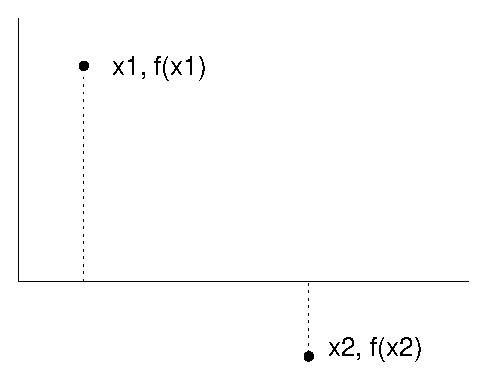
\includegraphics[height=1.5in]{figs/secant.eps}}

If this was all you knew about $f$, where would you go looking for
a zero? If you said ``halfway between $x_1$ and $x_2$,'' then
congratulations! You just invented a numerical method called
bisection!

If you said, ``I would connect the dots with a straight line
and compute the zero of the line,'' then
congratulations! You just invented the secant method!

And if you said, ``I would evaluate $f$ at a third point, find the
parabola that passes through all three points, and compute the zeros
of the parabola,'' then... well, you probably didn't say that.

Finally, if you said, ``I would use a built-in Octave function that
combines the best features of several efficient and robust
numerical methods,'' then you are ready to go on to the next section.


\section{{\tt fzero}}
\label{fzero}

{\tt fzero} is a built-in Octave function that
combines the best features of several efficient and robust
numerical methods.

In order to use {\tt fzero}, you have to define a Octave function
that computes the error function you derived from the original
nonlinear equation, and you have to provide an initial guess at
the location of a zero.

We've already seen an example of an error function:

\begin{verbatim}
function res = error_func(x)
  res = x.^2 - 2*x -3;
end
\end{verbatim}

You can call {\tt error\_func} from the Command Window, and
confirm that there are zeros at 3 and -1.

\begin{verbatim}
octave:1> error_func(3)
ans = 0

octave:2> error_func(-1)
ans = 0
\end{verbatim}

But let's pretend that we don't know exactly where
the roots are; we only know that one of them is between 0 and 4. Then
we could call {\tt fzero} like this:

\begin{verbatim}
octave:3> fzero(@error_func, [0, 4])
ans = 3
\end{verbatim}

Success! We found one of the zeros.

The first argument is a
{\bf function handle} that names the M-file that evaluates
the error function. The {\tt @} symbol allows us to name the
function without calling it. The interesting thing here is
that you are not actually calling {\tt error\_func} directly;
you are just telling {\tt fzero} where it is. In turn, {\tt fzero}
calls your error function---more than once, in fact.

The second argument is a vector that tells {\tt fzero} where we
guess the zero is. (The bracket operator is a convenient way 
(one of several) to create a new vector.) In this case, we know that
there's a root that's greater than 2 and less than 4.

You might be curious to know how many times {\tt fzero} calls your
function, and where. If you modify {\tt error\_func} so that it displays
the value of {\tt x} every time it is called and then run {\tt fzero}
again, you get:

\begin{verbatim}
octave:4> fzero(@error_func, [0,4])
x = 0
x = 4
x = 1.5000
x = 2.7500
x = 3.0000
x = 3.0000
x = 3.0000
x = 3
ans = 3
\end{verbatim}

Not surprisingly, it starts by computing $f(0)$ and $f(4)$. After
each iteration, the interval that brackets the root gets smaller;
{\tt fzero} stops when the interval is so small that the estimated
zero is correct to 16 digits. If you
don't need that much precision, you can tell {\tt fzero} to give
you a quicker, dirtier answer (see the documentation for details).


\section{What could go wrong?}

The most common problem people have with {\tt fzero} is leaving
out the {\tt @}. In that case, you get something like:

\begin{verbatim}
octave:1> fzero (error_func, [0, 4])
error: `x' undefined near line 2 column 8
error: called from:
error:   /home/gpleiss/Dropbox/Workspace/Octave/error_func.m at 
line 2, column 6
error: evaluating argument list element number 1
error: evaluating argument list element number 1
\end{verbatim}

Which is a very confusing error message. The problem is that Octave
treats the first argument as a function call, so it calls {\tt error\_func}
with no arguments. Since {\tt error\_func} requires one argument, the
message indicates that the input argument is ``undefined,'' although
it might be clearer to say that you haven't provided a value for it.

Probably the second most common error is providing a scalar instead of a vector
as {\tt fzero}'s second argument.

\begin{verbatim}
octave:1> x = fzero(@error_func, 4)
error: fzero: zero point is not bracketed
error: called from:
error:   /usr/share/octave/3.2.3/m/optimization/fzero.m at 
line 255, column 1
\end{verbatim}
 
This error message isn't as confusing as the last one, but it still doesn't
give you a good idea of what's going on. Always double check for the {\tt @}
sign and that you provided a vector for the initial guess. It will save you
hours of debugging!

Another common problem is writing an error function that never
assigns a value to the output variable. In general, functions should
{\em always} assign a value to the output variable, but Octave doesn't
enforce this rule, so it is easy to forget. For example, if you
write:

\begin{verbatim}
function res = error_func(x)
  y = x.^2 - 2*x -3
end
\end{verbatim}

and then call it from the Command Window:

\begin{verbatim}
octave:1> error_func(4)
y = 5
\end{verbatim}

It looks like it worked, but don't be fooled. This function assigns
a value to {\tt y}, and it displays the result, but when the function
ends, {\tt y} disappears along with the function's workspace.
If you try to use it with {\tt fzero}, you get

\begin{verbatim}
octave:2> fzero (@error_func, [0, 4])
y = -3
y =  5
y = -3
warning: error_func: some elements in list of return values 
are undefined
warning: error_func: some elements in list of return values 
are undefined
warning: error_func: some elements in list of return values 
are undefined
error: fzero: zero point is not bracketed
error: called from:
error:   /usr/share/octave/3.2.3/m/optimization/fzero.m at 
line 255, column 1
\end{verbatim}

You would have seen the same error message when you called {\tt
error\_func} from the interpreter, if only you had assigned the result
to a variable:

\begin{verbatim}
octave:2> x = error_func(4)
y =  5
x = [](0x0)
warning: error_func: some elements in list of return values 
are undefined
\end{verbatim}

You can avoid all of this if you remember these two rules:

\begin{itemize}

\item Functions should always assign values to their output
variables\footnote{Well, ok, there are exceptions, including {\tt
find\_triples}. Functions that don't return a value are sometimes
called ``commands,'' because they do something (like display values or
generate a figure) but either don't have an output variable or don't
make an assignment to it.}.

\item When you call a function, you should always do something with
the result (either assign it to a variable or use it as part of an
expression, etc.).

\end{itemize}

When you write your own functions and use them yourself, it is easy
for mistakes to go undetected. But when you use your functions with
Octave functions like {\tt fzero}, you have to get it right!

Yet another thing that can go wrong: if you provide an interval for the
initial guess that doesn't actually contain a root, you get

\begin{verbatim}
>>> x = fzero(@error_func, [0, 1])
error: fzero: not a valid initial bracketing
error: called from:
error:   /usr/share/octave/3.2.3/m/optimization/fzero.m 
at line 137, column 5
\end{verbatim}

This looks similar to the error message we got when we forgot to make the
initial guess a scalar, but it's a completely different error. In this case it
is not a bug in our code -- we just didn't provide a good interval.

{\tt fzero} is generally pretty robust, so you may never have a
problem, but you should remember that there is no guarantee that {\tt
fzero} will work.


\section{Finding an initial guess}

The better your initial guess (or interval) is, the more likely
it is that {\tt fzero} will work, and the fewer iterations it will
need.

When you are solving problems in the real world, you will usually
have some intuition about the answer. This intuition is often enough
to provide a good initial guess for zero-finding.

Another approach is to plot the function and see if you can
approximate the zeros visually. If you have a function, like
{\tt error\_func} that takes a scalar input variable and returns
a scalar output variable, you can plot it with {\tt ezplot}:

\begin{verbatim}
octave:1> ezplot(@error_func, [-2,5])
\end{verbatim}

The first argument is a function handle; the second is the 
interval you want to plot the function in.

By default {\tt ezplot} calls your function 100 times (each time
with a different value of {\tt x}, of course). So you probably want
to make your function silent before you plot it.

\section{More name collisions}

Functions and variables occupy the same ``name-space,'' which means
that whenever a name appears in an expression, Octave starts by looking
for a variable with that name, and if there isn't one, it looks for
a function.

As a result, if you have a variable with the same name as a function,
the variable {\bf shadows} the function. For example, if you assign
a value to {\tt sin}, and then try to use the {\tt sin} function, you
{\em might} get an error:

\begin{verbatim}
octave:1> sin = 3;
octave:2> x = 5;
octave:3> sin(x)
error: A(I): Index exceeds matrix dimension.
\end{verbatim}

In this example, the problem is clear. Since the value of {\tt sin}
is a scalar, and a scalar is really a 1x1 matrix, Octave tries to
access the 5th element of the matrix and finds that there isn't one.
Of course, if there were more distance between the assignment
and the ``function call,'' this message would be pretty confusing.

But the only thing worse than getting an error message is {\em not}
getting an error message. If the value of {\tt sin} was a vector,
or if the value of {\tt x} was smaller, you would really
be in trouble.

\begin{verbatim}
octave:3> sin = 3;
octave:4> sin(1)
ans = 3
\end{verbatim}

Just to review, the sine of 1 is not 3!

The converse error can also happen if you try to access an
undefined variable that also happens to be the name of a function.
For example, if you have a function named {\tt f}, and then
try to increment a variable named {\tt f} (and if you forget to
initialize {\tt f}), you get

\begin{verbatim}
octave:5> f = f+1
error: `x' undefined near line 2 column 12
error: evaluating argument list element number 1
error: called from:
error:   /home/gpleiss/Octave/f.m at line 2, column 6
\end{verbatim}

There is no universal way to avoid these kind of
collisions, but you can improve your chances by choosing
variable names that don't shadow existing functions, and by
choosing function names that you are unlikely to use as variables.
That's why in Section~\ref{notation} I called the error function
{\tt error\_func} rather than {\tt f}. I often give functions
names that end in {\tt func}, so that helps, too.


\section{Debugging in four acts}

When you are debugging a program, and especially if you are
working on a hard bug, there are four things to try:

\begin{description}

\item[reading:] Examine your code, read it back to yourself, and
check that it means what you meant to say.

\item[running:] Experiment by making changes and running different
versions. Often if you display the right thing at the right place
in the program, the problem becomes obvious, but sometimes you have to
spend some time to build scaffolding.

\item[ruminating:] Take some time to think! What kind of error
is it: syntax, run-time, logical? What information can you get from
the error messages, or from the output of the program? What kind of
error could cause the problem you're seeing? What did you change
last, before the problem appeared?

\item[retreating:] At some point, the best thing to do is back
off, undoing recent changes, until you get back to a program that
works, and that you understand. Then you can starting rebuilding.

\end{description}

Beginning programmers sometimes get stuck on one of these activities
and forget the others. Each activity comes with its own failure
mode.

For example, reading your code might help if the problem is a
typographical error, but not if the problem is a conceptual
misunderstanding. If you don't understand what your program does, you
can read it 100 times and never see the error, because the error is in
your head.

Running experiments can help, especially if you run small, simple
tests. But if you run experiments without thinking or reading your
code, you might fall into a pattern I call ``random walk programming,''
which is the process of making random changes until the program
does the right thing. Needless to say, random walk programming
can take a long time.

The way out is to take more time to think. Debugging is like an
experimental science. You should have at least one hypothesis about
what the problem is. If there are two or more possibilities, try to
think of a test that would eliminate one of them.

Taking a break sometimes helps with the thinking. So does talking.
If you explain the problem to someone else (or even yourself), you
will sometimes find the answer before you finish asking the question.

But even the best debugging techniques will fail if there are too many
errors, or if the code you are trying to fix is too big and
complicated. Sometimes the best option is to retreat, simplifying the
program until you get to something that works, and then rebuild.

Beginning programmers are often reluctant to retreat, because
they can't stand to delete a line of code (even if it's wrong).
If it makes you feel better, copy your program into another file
before you start stripping it down. Then you can paste the pieces
back in a little bit at a time.

To summarize, here's the Ninth Theorem of debugging:

\begin{quote}
Finding a hard bug requires reading, running, ruminating, and
sometimes retreating. If you get stuck on one of these activities,
try the others.
\end{quote}



\section{Glossary}

\begin{description}

\item[analytic solution:] A way of solving an equation by performing
algebraic operations and deriving an explicit way to
compute a value that is only known implicitly.

\item[numerical solution:] A way of solving an equation by finding
a numerical value that satisfies the equation, often approximately.

\item[numerical method:] A method (or algorithm) for generating
a numerical solution.

\item[map:] A correspondence between the elements of one set (the
range) and the elements of another (the domain). You can think of
sequences, vectors and functions as different kinds of maps.

\item[range:] The set of values a map maps from.

\item[domain:] The set of values a map maps to.

\item[discrete set:] A set, like the integers, whose elements are
countable.

\item[continuous set:] A set, like the real numbers, whose elements
are not countable. You can think of floating-point numbers as a
continuous set.

\item[zero (of a function):] A value in the range of a function that
maps to 0.

\item[function handle:] In Octave, a function handle is a way of
referring to a function by name (and passing it as an argument)
without calling it.

\item[shadow:] A kind of name collision in which a new definition
causes an existing definition to become invisible. In Octave,
variable names can shadow built-in functions (with hilarious results). 

\end{description}

\section{Exercises}

\begin{ex}

\begin{enumerate}

\item Write a function called {\tt cheby6} that evaluates the
6th Chebyshev polynomial. It should take an input variable, 
$x$, and return

\begin{equation}
32 x^6 - 48 x^4 + 18 x^2 - 1
\end{equation}

\item Use {\tt ezplot} to display a graph of this function in the
interval from 0 to 1. Estimate the location of any zeros in this
range.

\item Use {\tt fzero} to find as many different roots as you can.
Does {\tt fzero} always find the root that is closest to the initial
guess?

\end{enumerate}
\end{ex}


\begin{ex}
\label{duck}

The density of a duck, $\rho$, is $0.3 g / cm^3$ (0.3 times the
density of water).

The volume of a sphere\footnote{This example is adapted from Gerald
and Wheatley, {\em Applied Numerical Analysis}, Fourth Edition,
Addison-Wesley, 1989.} with radius $r$ is $\frac{4}{3} \pi r^3$.

If a sphere with radius $r$ is submerged in water to a depth $d$, the
volume of the sphere below the water line is 

\[ volume = \frac{\pi}{3} (3r d^2 - d^3) \quad 
\mbox{as long as} \quad d < 2 r \]

An object floats at the level where the weight of the displaced water
equals the total weight of the object.

Assuming that a duck is a sphere with radius 10 cm, at what depth does
a duck float?

Here are some suggestions about how to proceed:

\begin{itemize}

\item Write an equation relating $\rho$, $d$ and $r$.

\item Rearrange the equation so the right-hand side is zero.
Our goal is to find values of $d$ that are roots of this equation.

\item Write a Octave function that evaluates this function. Test it,
  then make it a quiet function.

\item Make a guess about an interval that contains $d$. It can be a big
interval if you want.

\item Use {\tt fzero} to find a root in your interval.

\item Check to make sure the result makes sense. In particular,
  check that $d < 2 r$, because otherwise the volume equation
  doesn't work!

\item Try different values of $\rho$ and $r$ and see if you get the
effect you expect. What happens as $\rho$ increases? Goes to
infinity? Goes to zero? What happens as $r$ increases? Goes to
infinity? Goes to zero?

\end{itemize}


\end{ex}

% for another time, figure out how to use fzero to find zeros of...

%\item The Riemann zeta function can be written

%\[ zeta \equiv w \to sum_{k=1}^\infty k^w \]

%where $w$ is a complex number. If you are not familiar with
%complex numbers, you should skip this problem.
